%camera placement and positioning reference: http://www.lorextechnology.com/support/self-serve/Camera-Location-Placement-and-Positioning/2700036
The purpose of the web cameras is simply to surveillance the area they have been placed in and forward the captured frames to Raspberry Pi computers for further processing, as shown in Figure~\ref{fig:system_overview}. The cameras can be placed in a room, corridor, atrium or any other similar place in or outside of the building, where the services offered are required. Cameras can be placed either directly above the observed area, as shown in Figure~\ref{fig:camera_top} or in the corner of it, as illustrated in Figure~\ref{fig:camera_corner}. Naturally, a camera placed above the observed area would give better results, since this increases its field of view and this makes it easier to correctly detect and distinguish between multiple people walking side by side. Furthermore, for the best results one must also take many different factors into account, such as the distance between the camera and monitored area, environmental conditions of the area the camera is placed in, and lighting conditions.

% Camera top placement.
\begin{figure}[ht]
	\centering
	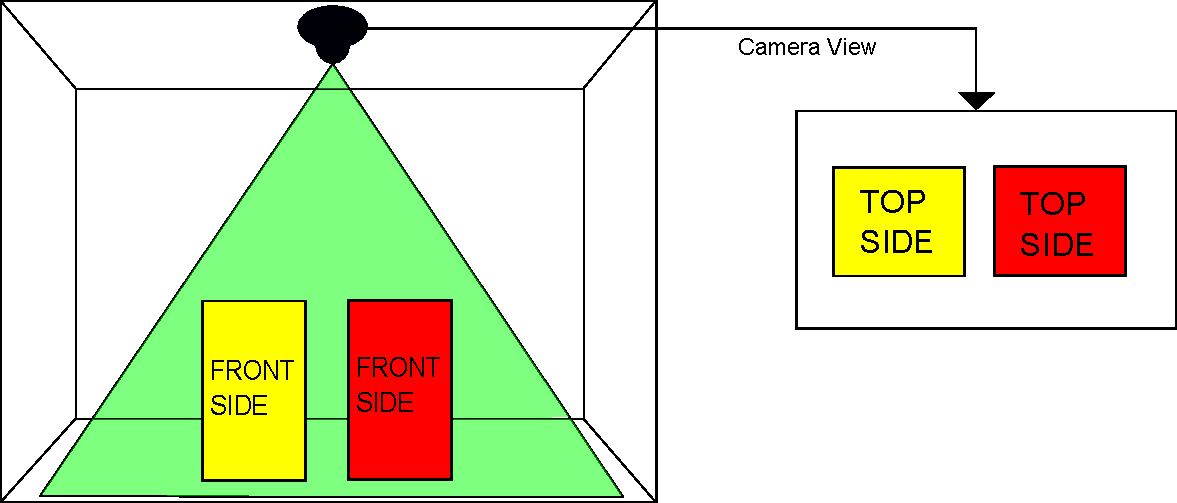
\includegraphics[scale=0.82]{camera_placement/camera_top}
	\caption{Camera top placement}
	\label{fig:camera_top}
\end{figure}

% Camera corner placement.
\begin{figure}[ht]
	\centering
	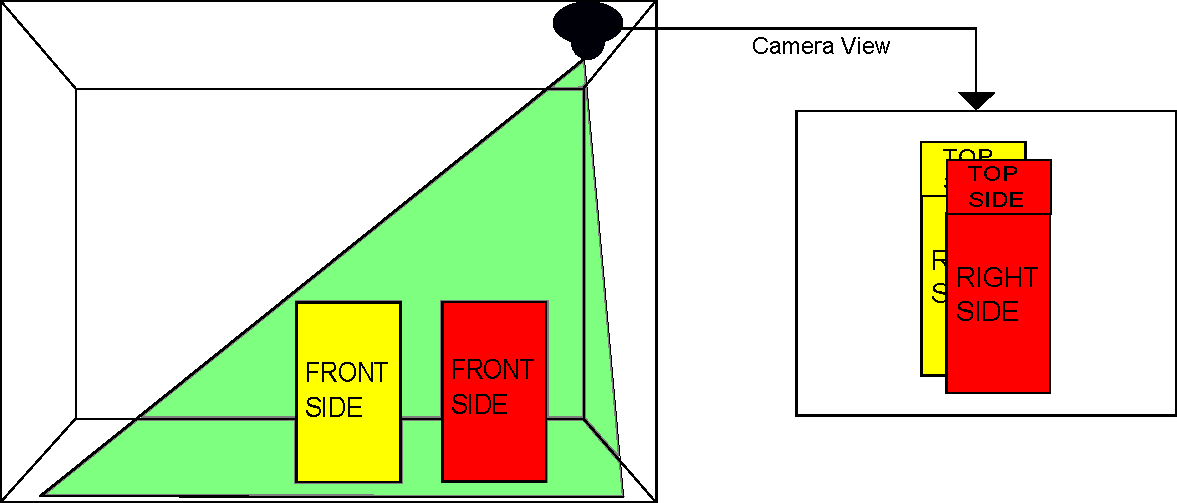
\includegraphics[scale=0.82]{camera_placement/camera_corner}
	\caption{Camera corner placement}
	\label{fig:camera_corner}
\end{figure}